\documentclass[hyperref={pdfpagelabels=false}]{beamer}
\setbeamercolor{background canvas}{bg=white}
\usepackage{graphicx,lmodern,subfigure,ulem,color,graphicx,tikz,booktabs,natbib}
\usepackage{mathrsfs}
\usetheme{Warsaw}
%\definecolor{beamer@blendedblue}{rgb}{0.1,0.5,0.1}
%\definecolor{ForestGreen}{RGB}{60, 140, 60}
%\setbeamercolor{structure}{fg=beamer@blendedblue}
\setbeamertemplate{navigation symbols}{}
\setbeamertemplate{footline}[frame number]
\bibliographystyle{chicago}
\newcommand{\spitem}{\vspace{.3cm}\item}
\newcommand{\elas}{$E_{labor}$}
\def \ourFigPath {../../} 

\usetheme[
outer/progressbar=foot,
outer/numbering=none
]{metropolis}



\title{Putting the Cycle Back into Business Cycle Analysis}
\author{Beaudry, Galizia, and Portier (forthcoming AER)}
\institute{Macro Reading Group, Boston College}
\date{February 2019}


\begin{document}
	
	\frame{
		
		
		\maketitle
}



\frame{\frametitle{Business Cycle Analysis and Modern Macroeconomics}
	
Forces and mechanisms that drive economic fluctuations remain a debated subject. 


\

Two theoretical approaches:
	
	
	\begin{enumerate}
		\item BCs are primarily driven by persistent exogenous shocks
		
		
		\item BCs are mostly driven by forces internal to the economy which endogenously favor recurrent periods of boom and bust.
	\end{enumerate}   

\

This paper argues that data favors the second theoretical approach. 
		
}

\frame{\frametitle{Appeals of the First Approach}
	
	\begin{enumerate}
		\item Empirical estimation of DSGE models support the existence and the persistence of exogenous driving forces to explain the data. 
		
		\
		
		\
		
		\item Since Granger (1966) and Sargent (1987), it has been argued that data are generally not supportive of strong internal boom-bust mechanisms.
	\end{enumerate}
	
		
}

\frame{\frametitle{This Paper}
	
\begin{enumerate}
	\item They examine spectral density properties of macro aggregates
	\begin{itemize}
		\item a recurrent peak in several spectral densities at periodicities around 9 to 10 years
	\end{itemize}

\


	\item They analyze necessary features to theoretically reproduce peaks in the spectral densities
	\begin{itemize}
		\item strategic complementaries across agents
		\item accumulation of a stock with decreasing returns 
	\end{itemize}

\


	\item They estimate a NK model where persistent shocks and endogenous cyclical mechanisms compete to explain data
	\begin{itemize}
	\item estimation favors endogenous mechanisms to match empirical spectral density 
	\item estimation suggests the existence of stochastic limit cycles 
\end{itemize}	
\end{enumerate}
	
	
}
	

\frame{\frametitle{Empirical Evidence - NBER Recessions}
	
\begin{center}
	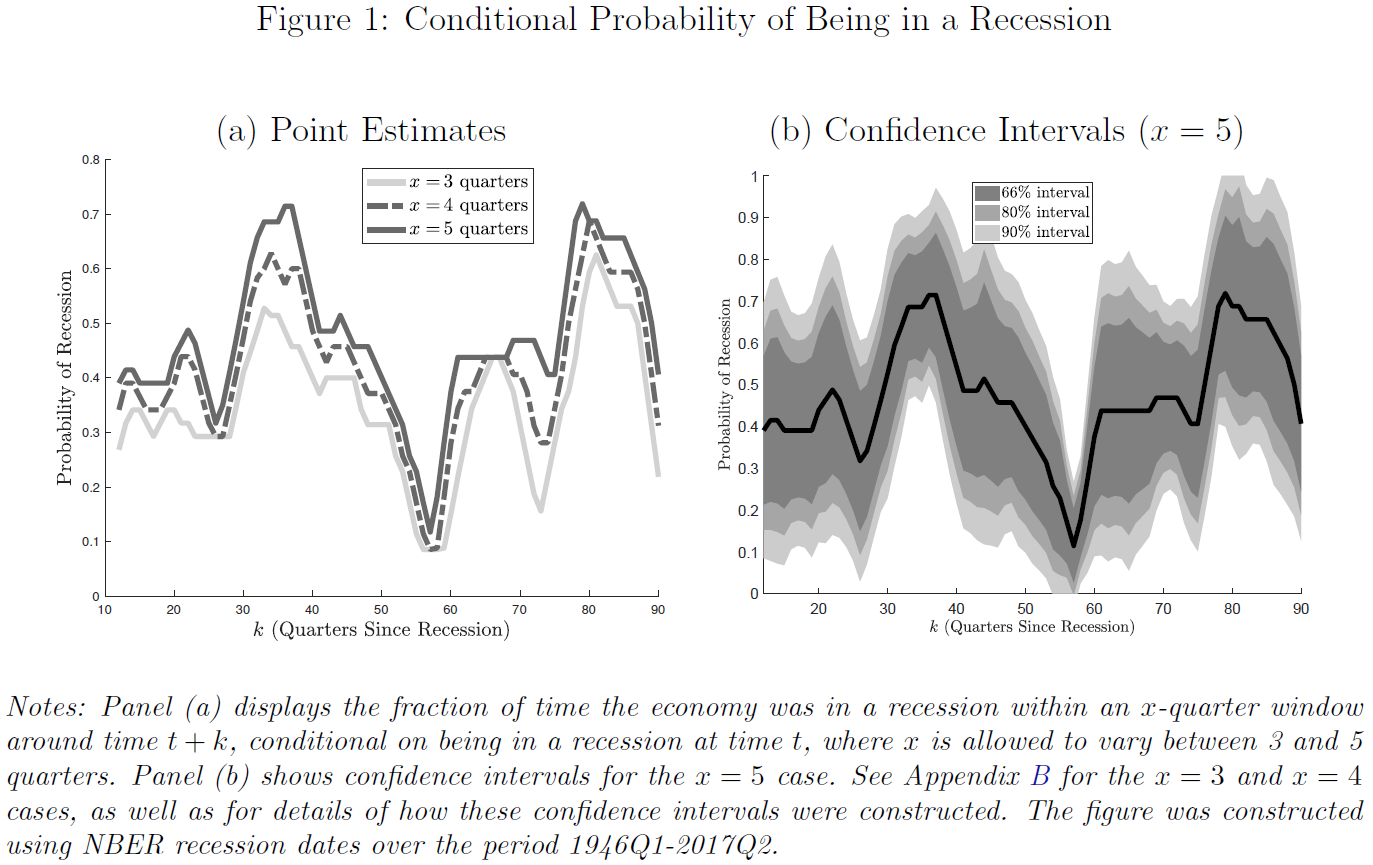
\includegraphics[scale=0.3]{NBER}
\end{center}
	
}


\frame{\frametitle{Empirical Evidence (II) - Hours Worked per Capita}
	

\begin{center}
	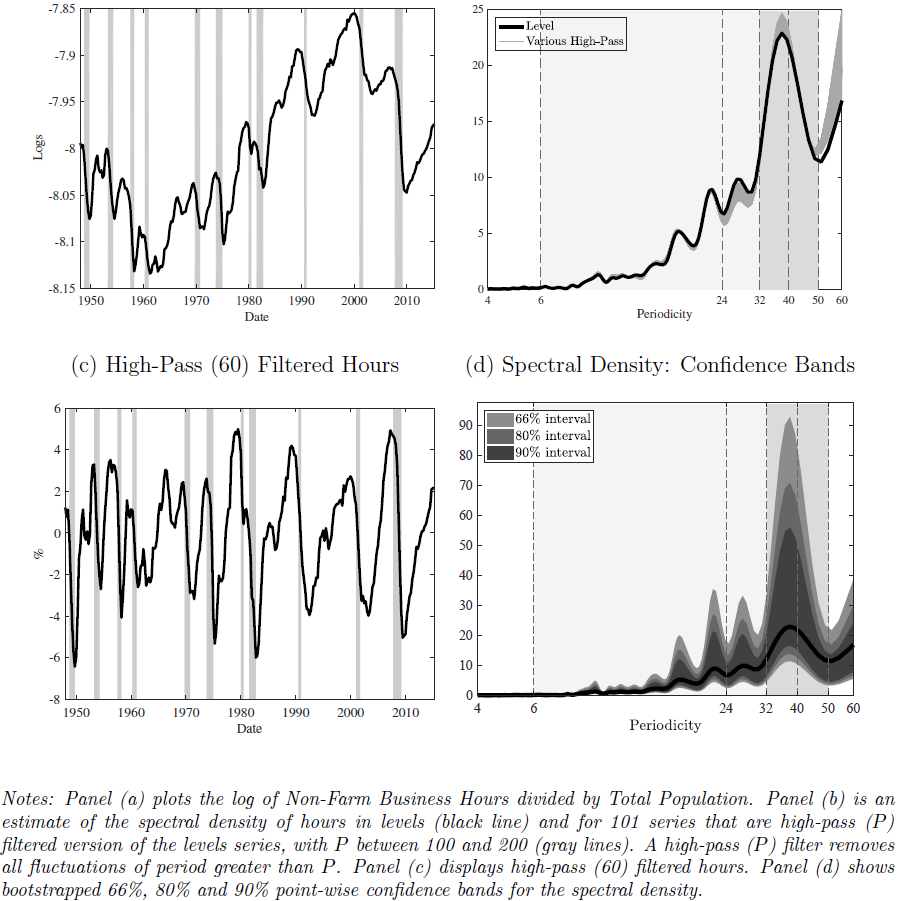
\includegraphics[scale=0.4]{spectrum_four}
\end{center}

}

\frame{\frametitle{Empirical Evidence (II) - Financial Variables}
	
	\begin{center}
		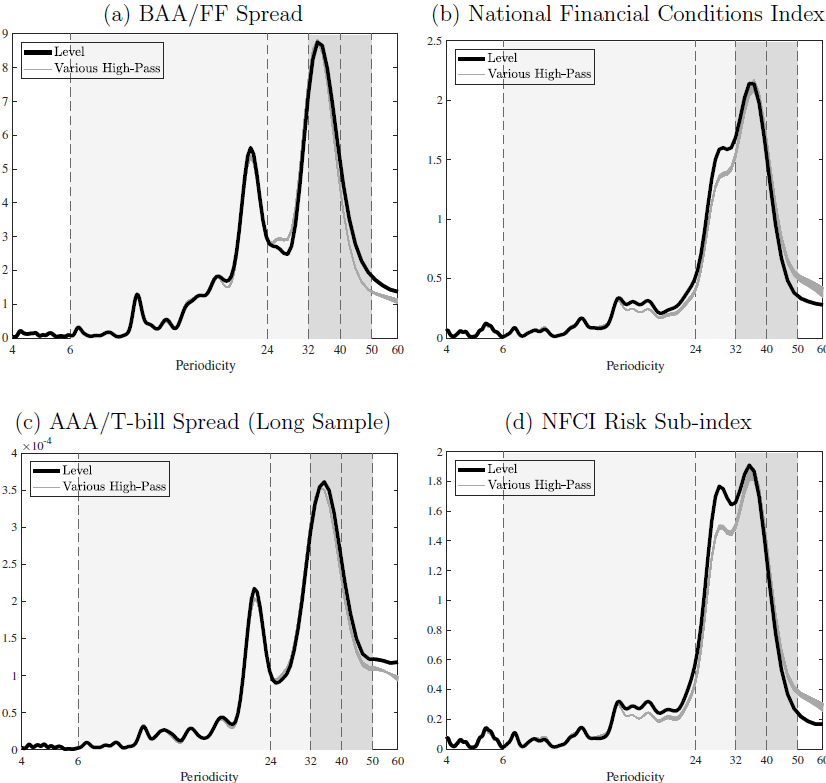
\includegraphics[scale=0.38]{financial}
	\end{center}
	
	
}


\frame{\frametitle{Spectra Implied by Current DSGE Models}
	
	\begin{center}
		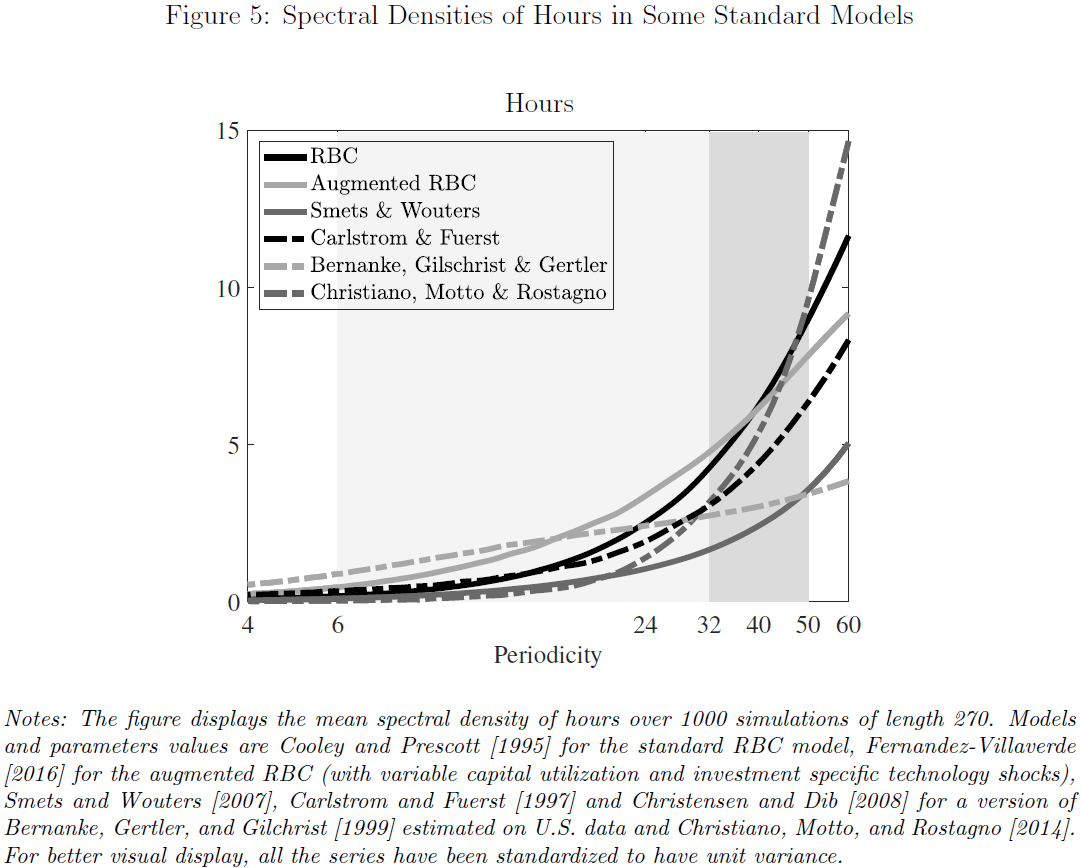
\includegraphics[scale=0.34]{DSGE_fail}
	\end{center}
	

}






\frame{\frametitle{Takeaway}

\begin{itemize}
	\item Probability to fall in a recession rises every 8-10 years
	\item Measures of labor activity exhibit significant spectral peaks at a periodicity of around 36-40 quarters
	\item Financial variables display analogous patters
	\item Current theoretical models are unable to match previous facts
	\end{itemize}

\

They provide a class of models able to reproduce cyclical outcomes based on equilibrium interactions internal to the model.
	

	
}

\frame{\frametitle{A Class of Models}
	
Consider an environment with $N$ agents indexed by $j$.

\

Agent $j$ makes decision $e_{j,t}$ according to,
\begin{eqnarray}
e_{j,t} = \alpha_1 X_{j,t} + \alpha_2 e_{j,t-1} + \alpha_3 q_t + \mu_t, \ \ \ 0 < \alpha_2 < 1
\end{eqnarray}
where is $X_t$ is a stock variable with the following law of motion,
\begin{eqnarray}
X_{j,t+1} = (1 - \delta) X_{j,t} + e_{j,t}, \ \ \ 0 < \delta < 1
\end{eqnarray}
and $\mu_t$ is an exogenous driving force. Finally, $q_t$ is a aggregate market determined variable,
\begin{eqnarray}
q_t = \alpha_4 \frac{1}{N} \sum_j e_{j,t} = \alpha_4 e_{t}
\end{eqnarray}
where $\alpha_3 \alpha_4$ governs the degree of strategic complementarity (substitutability) in the economy.


}


\frame{\frametitle{Spectrum of $e_t$}
	
	Invoke symmetry and solve for $e_t$,
	\begin{eqnarray*}
	e_t = \bigg( \frac{\alpha_1 + \alpha_2}{1 - \alpha_3 \alpha_4} + 1 - \delta \bigg)e_{t-1} - \frac{\alpha_2(1-\delta)}{1 - \alpha_3 \alpha_4} e_{t-2} + \frac{1-(1-\delta)L}{1 - \alpha_3\alpha_4}\mu_t
	\end{eqnarray*}
	which implies the following spectral density
	\begin{eqnarray*}
    s_e(\omega) = s_{\mu}(\omega) \frac{[1 - (1 -\delta)\exp(i\omega)][1 - (1 -\delta)\exp(i\omega)]}{(1 - \alpha_3 \alpha_4)^2}g(\omega)
    \end{eqnarray*}
	where 
	\begin{itemize}
		\item $g(\omega) \equiv [B(\exp(i\omega)) B(\exp(i\omega))]^{-1}$
	    \item $B(L) \equiv 1 - \Big( \frac{\alpha_1 + \alpha_2}{1 - \alpha_3 \alpha_4} + 1 - \delta \Big)L + \frac{\alpha_2(1-\delta)}{1 - \alpha_3 \alpha_4}L^2$
	\end{itemize}
}



\frame{\frametitle{Necessary Conditions for Peak in the Spectral Density}


Sargent (1979): necessary conditions is $B(L)$ to have complex roots in $L$.

\

Assumption: parameters are such that if $\alpha_3 \alpha_4 = 0$, then the eigenvalues are real, positive and smaller than 1.


Then, necessary conditions are
\begin{itemize}
	\item $\alpha_3 \alpha_4 > 0$: strategic complementarity
	\item $\alpha_1 < 0$: decreasing returns in $X_{j,t}$
\end{itemize}

\begin{eqnarray*}
\begin{cases}
e_{j,t} = \alpha_1 X_{j,t} + \alpha_2 e_{j,t-1} + \alpha_3 \alpha_4 e_t + \mu_t \\
X_{j,t+1} = (1 - \delta) X_{j,t} + e_{j,t}
\end{cases}
\end{eqnarray*}

}



\frame{\frametitle{Technical Ingredients}
	
	In order to have a peak in the spectral density which is not driven by exogenous forces, they need 
	
	
	\begin{itemize}
		\item Complex eigenvalues 
		\begin{itemize}
			\item Dynamics are represented by trigonometric functions
			\item For an AR(2) process complex eigenvalues are a necessary condition for a peak in the spectral density (Sargent, 1979)
		\end{itemize}
		
		\
		
		
		\item Local instability surrounded by a stochastic limit cycle 
		\begin{itemize}
			\item Cyclical dynamics are perpetual
			\item Main critique of limit cycle dynamics: predictability and regularity of the cycle
			\item However, when a limit cycle is perturbed by unpredictable disturbances, size and period of the cycle changes permanently
		\end{itemize}
	\end{itemize} 
	

}

\frame{
	\frametitle{Economic Ingredients}
	
		In order to have a peak in the spectral density which is not driven by exogenous forces, they need 
	

	
	\begin{itemize}
		\item Strategic complementarity 
		\begin{itemize}
			\item It is a well-known source of instability
		\end{itemize}
		
		\
		
		
		\item Decreasing return in a stock variable 
				\begin{itemize}
			\item When combined with strategic complementarity, the economy exhibits periods of accumulation and dissipation.
		\end{itemize}
	\end{itemize} 


}

\frame{\frametitle{A New Keynesian Model}


Augment a standard NK Model with
\begin{itemize}
	\item External habit formation
	\item Intra-temporal budget constraint on the household side
	\item Positive and endogenous probability of bankruptcy 
	\item Lender cannot fully recover its investment after bankruptcy
\end{itemize}







}



\frame{\frametitle{Household}
	
	Household $h$'s preferences are given by
	\begin{eqnarray}
	E_0 \sum_t \beta^t \zeta_{t-1} [U(C_{h,t} - \gamma C_{t-1}) + \nu (1 - e_{h,t})]
	\end{eqnarray}
    In addition to purchase consumption services $C_{h,t}$ at price $P_t$ and labor $e_{h,t}$ at wage $W_t$, household $h$ decides to purchase an amount $I_t$ of durable consumption $X_{h,t}$ at price $P_t^X$.
    
    \
    
    Law of motion of $X_{h,t}$ is: 
    $$
    X_{h,t+1} = (1 - \delta)X_{h,t} + I_t
    $$
    and household budget constraint is: 
    $$
    \underbrace{(1 + i_t)}_{\text{Deposit Rate}} Y_{h,t} \geq \underbrace{[e_t + (1 - e_t)\phi]}_{\text{Prob. of Repay}}\underbrace{(1+r_t)}_{\text{Risky Rate}}\underbrace{(P_tC_{h,t} + P_t^X I_{h,t})}_{\text{Loan}}
    $$


}

\frame{\frametitle{Banks}
	
	Households have to pay in advance purchases of consumption services ($C_{h,t}$) and durable goods ($I_{h,t}$).
	
	
	
	Banks finance household purchases at interest rate $1 + r_t$ which satisfies the following zero-profit condition
	\begin{eqnarray*}
	1 + r_t = (1 + i_t) \frac{1 + (1 - e_t)\phi \Phi}{e_t + (1 - e_t)\phi}
	\end{eqnarray*}
	where risk premium is
		\begin{eqnarray}
	1 + r_t^p = \frac{1 + (1 - e_t)\phi \Phi}{e_t + (1 - e_t)\phi}
	\end{eqnarray}
	
	
	
}

\frame{\frametitle{Firms}


Intermediate firm $k$ produces consumption services as follows,
$$
C_{k,t} = s[X_{k,t} + \theta F(e_{k,t})], \ \ \ s > 0
$$
where $\theta$ is exogenous productivity. 

\

Moreover, the market for intermediate services is subject to sticky prices \`a la Calvo (1983).

\

Accordingly, final goods sector is competitive and combine $k$-specific consumption of services according to a Dixit-Stiglitz aggregator. 
	
	
}

\frame{\frametitle{Central Bank and Equilibrium}
	
	
	To close the model, central bank determine the risk-free rate $i_t$ according to
	$$
	1 + i_t = \Theta E_t [e_{t+1}^{\varphi_e} (1 + \pi_{t+1})]
	$$
	
	\
	
	Equilibrium is defined as
		\begin{eqnarray}
	X_{t+1} = (1-\delta)X_t + \psi \theta F(e_t)
	\end{eqnarray}
			\begin{eqnarray}
			\begin{aligned}
		 & U'\{s[X_t + \theta F(e_t)]  - \gamma s [X_{t-1} + \theta F(e_{t-1})] \} \\
		  = \ &  (1 + (1 - e_t)\phi \Phi) \beta \frac{\zeta_t}{\zeta_{t-1}}\Theta \\
		   \times \ & E_t \big[  \{s[X_t + \theta F(e_t)]  - \gamma s [X_{t-1} + \theta F(e_{t-1})] \}  e_{t+1}^{\varphi_e}\big]
			\end{aligned}
	\end{eqnarray}
}

\frame{\frametitle{Economic Intuition}
	
	

\begin{itemize}
	\item Suppose to be in a recession
	\item Unemployment is high, so bankruptcy rate
	\item Risk premium is large and household consumption is low
	\item Capital $X_t$ is keep decreasing during this phase
	\item The lower $X_t$ the larger the marginal utility of the household
	\item MU will eventually be so high to be larger than the loan rate
	\item Household increases borrowings, increasing the demand
	\item Unemployment thus decrease, so does the bankruptcy rate
	\item Risk premium decreases, consumption and $X_t$ increase
	\item Capital $X_t$ is keep increasing during this phase
	\item The higher $X_t$ the lower the marginal utility of the household
	\item MU will eventually be so low to be lower than the loan rate
	\item \dots
\end{itemize}






}


\frame{\frametitle{Estimation of the Model}
	
	Exogenous parameters:
	\begin{itemize}
\item $\delta = 0.05$
\item $\alpha = 2/3$
\item $\Theta$ such that steady state unemployment rate is $0.0583$
\end{itemize}
	
	\
	
	\
	
	They estimate the remaining parameters (10) of the model via spectral density matching.
	
	
}

\frame{\frametitle{Estimation Results - Endogenous Parameters}
	
	\begin{center}
		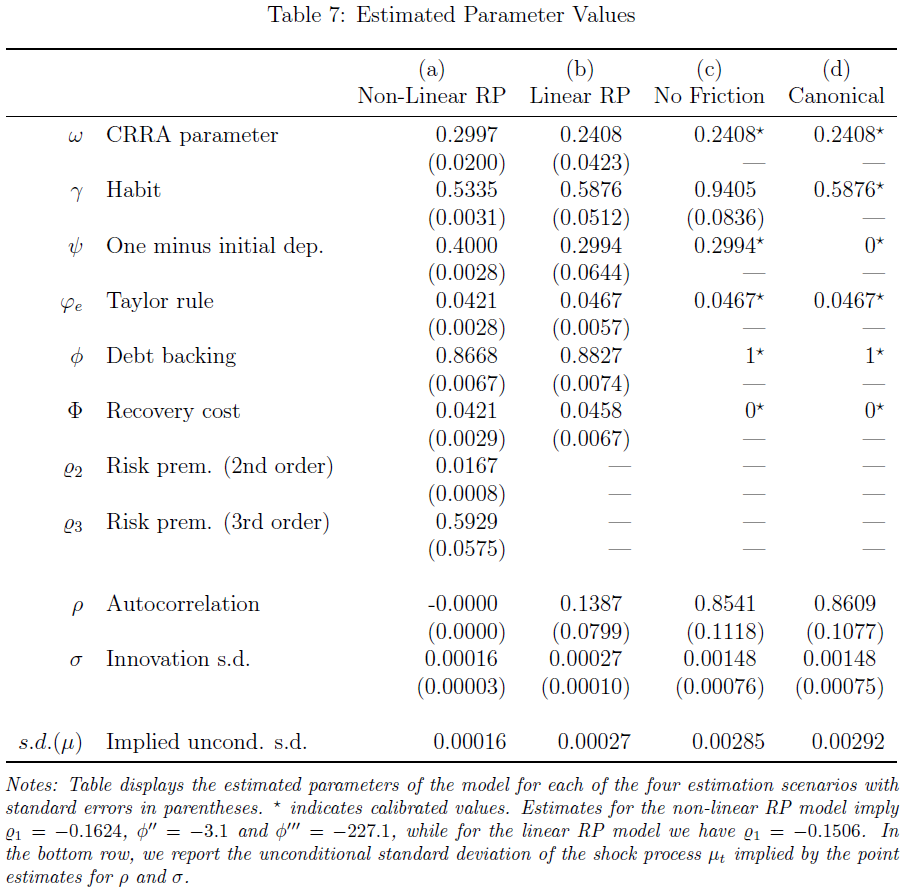
\includegraphics[scale=0.34]{param}
	\end{center}
	
	
}

\frame{\frametitle{Estimation Results - Eigenvalues}
	
	Solving the model with a less restrictive solution method allows to obtain  a parameterization that supports limit cycle and local instability
	
	\begin{center}
		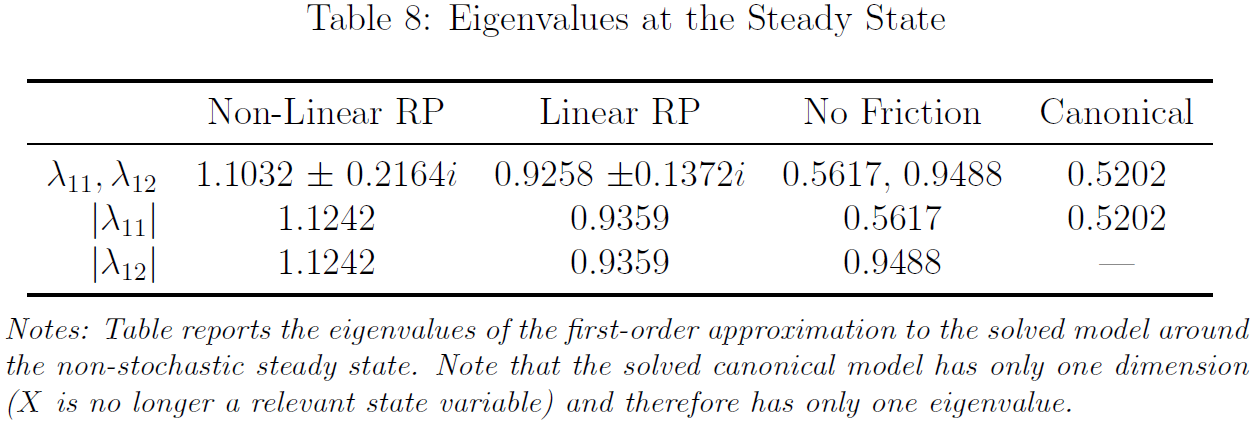
\includegraphics[scale=0.34]{eigen}
	\end{center}	
	
}


\frame{\frametitle{Estimation Results - Spectral Density}
	
	\begin{center}
		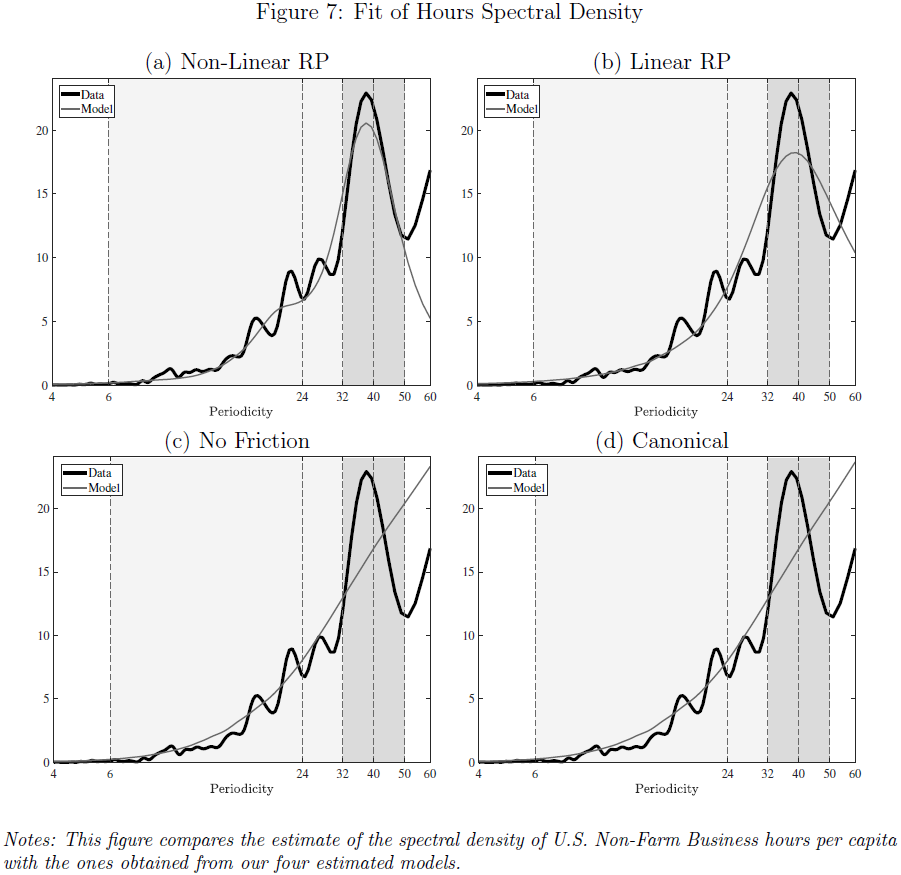
\includegraphics[scale=0.34]{matching}
	\end{center}
	
	
}



\frame{\frametitle{Conclusions}
	
Why do market economies experience business cycle?

\begin{itemize}
	\item Persistent outside disturbance
	\item Internal forces that endogenously favor cyclical outcomes
\end{itemize}

This paper:

\begin{itemize}
	\item Macro variables display predictable cyclical dynamics
	\item Strategic complementarity is key to match empirical properties of spectral density
	\item Models do not need large and persistent shocks to match observable features in the data
\end{itemize}
	
	
}



\end{document}









\end{document}